\documentclass[]{article}

% include Packages
%\usepackage{pdfpages}
\usepackage{amsmath,amssymb}
\usepackage{amsthm}
\usepackage{xcolor}
\usepackage{graphicx}
\usepackage{float}

% Formatting text ranges
\setlength{\textwidth}{450pt}
\setlength{\textheight}{685pt}
\setlength{\topmargin}{-40pt}
\setlength{\hoffset}{-15mm}

% Define Theorem environments
\newtheorem{theorem}{Theorem}
\newtheorem*{theorem*}{Theorem} % allow not enumerated theorems
\newtheorem{definition}{Definition}
\newtheorem{remark}{Remark}
\newtheorem{lemma}{Lemma}
\newtheorem{corollary}{Corollary}

% Define custom commands
\newcommand{\yopt}{y^*}
\newcommand{\todo}{{\color{red} TODO!}}
\newcommand{\ind}[2]{{#1}_{\mathrm{#2}}}
\newcommand{\trp}{^T}
\newcommand{\fx}{f(x)}
\newcommand{\fsigx}{f(\sigma x)}
\newcommand{\fxtrp}{f \trp (x)}
\newcommand{\xone}{x_1}
\newcommand{\xtwo}{x_2}
\newcommand{\dotx}{\dot x}
\newcommand{\dotxone}{\dotx_1}
\newcommand{\dotxtwo}{\dotx_2}
\newcommand{\Rn}{\mathbb{R}^n}
\newcommand{\Nset}{\mathbb{N}}
\newcommand{\forntoinf}{\overset{n \rightarrow \infty}{\longrightarrow}}
\newcommand{\jacf}{\dfrac{\partial }{\partial x} \fx}
\renewcommand{\brack}[1]{\left[ #1 \right]}
\newcommand{\parenth}[1]{\left( #1 \right)}
\newcommand{\jacfbrack}{\brack{\jacf}}
\newcommand{\matleq}{\preccurlyeq}
\newcommand{\norm}[1]{\parallel \! \! #1 \! \! \parallel}
\newcommand{\partialx}{\frac{\partial}{\partial x}}
\newcommand{\dsig}{\mathrm{d} \sigma}
\newcommand{\intsigma}{\int_{0}^{1} \partialx \fsigx x \dsig}
\newcommand{\Qx}{Q(x)}
\newcommand{\Vx}{V(x)}
\newcommand{\xtrp}{x \trp}
\newcommand{\gammaxsig}{\gamma(x,\sigma)}
\newcommand{\xn}{x_n}
\newcommand{\xnull}{x_0}
\newcommand{\unull}{u_0}
\newcommand{\xN}{x_N}
\newcommand{\xk}{x_k}
\newcommand{\uk}{u_k}
\newcommand{\xtrpn}{x_n \trp}
\newcommand{\fxn}{f(\xn)}
\newcommand{\dotVx}{\dot{V}(x)}
\newcommand{\dVdtx}{\frac{\mathrm{d} V(x)}{\mathrm{d} t}}
\newcommand{\partialVx}{\frac{\partial V(x)} {\partial x}}
\newcommand{\matricks}[4]{\begin{pmatrix}#1 & #2 \\ #3 & #4 \end{pmatrix}}
\newcommand{\twovector}[2]{\begin{pmatrix}{ #1 }\\{ #2 }\end{pmatrix}}
\newcommand{\Ad}{A_d}
\newcommand{\Bd}{B_d}
\newcommand{\xkplus}{x_{k+1}}
%\newcommand{\dotx}{\dot{x}}
\newcommand{\tk}{t_{k}}
\newcommand{\tkplus}{t_{k+1}}
\newcommand{\Aeul}{\ind{A}{eul}}
\newcommand{\Beul}{\ind{B}{eul}}
\newcommand{\optmin}{\mathrm{min}.}
\newcommand{\Aeq}{\ind{A}{eq}}
\newcommand{\beq}{\ind{b}{eq}}
\newcommand{\Aeqx}{\Aeq^x}
\newcommand{\Aequ}{\Aeq^u}
\newcommand{\Aineq}{\ind{A}{{  in}}}
\newcommand{\bineq}{\ind{b}{{  in}}}
\newcommand{\xbar}{\bar{x}}
\newcommand{\xtilde}{\tilde{x}}
\newcommand{\vectorthree}[3]{\begin{pmatrix}
		#1 \\ #2 \\ #3
\end{pmatrix}}
\newcommand{\vectortwo}[2]{\begin{pmatrix}
		#1 \\ #2
\end{pmatrix}}
\newcommand{\half}{\frac{1}{2}}
\newcommand{\grad}{\nabla}
\newcommand{\N}{\mathbb{N}}
\newcommand{\R}{\mathbb{R}}
%\newcommand{\Rn}{\mathbb{R}^n}
\newcommand{\Rm}{\mathbb{R}^m}
\newcommand{\Rp}{\mathbb{R}^p}
\newcommand{\Fx}{F(x)}
\newcommand{\jac}{J}
\newcommand{\jacF}{\jac F}
\newcommand{\inv}{^{-1}}

%opening
\title{Optimal Control WS20/21: Homework 1}
\author{Daniel Bergmann}

\begin{document}

\maketitle

\section{Theory Part}
First, all answers to theoretical questions are given. The regarding plots can be found in section \ref{sec:plots}.
\begin{enumerate}
	\item[\bf a)] Discretize cost functional:\\
		Discretizing  with time step size $ h $ \[ \xk \overset{\mathrm{def}}{=} x(kh) \overset{\mathrm{def}}{=} x(t_k) \] and evaluate the running cost at each $ t_k $ for all $ k = 0,\dots,N $. This yields
	 	\begin{equation}
			 J \approx  \xN\trp Q \xN + \sum_{k = 0}^{N-1} \xk \trp Q \xk + \uk\trp R \uk.
	 	\end{equation}
		
	\item[\bf b)] Matrix representation of discretized linear dynamics:\\
	
	We know
	\begin{equation}
		x(t) = e^{At} x(0) + \int_{0}^{t} e^{A(t-\tau)} B u(\tau) d\tau \label{eq:varofconst}
	\end{equation}
		Discretizing  with time step size $ h $ \[ \xk \overset{\mathrm{def}}{=} x(kh) \overset{\mathrm{def}}{=} x(t_k) \] and inserting it into  \eqref{eq:varofconst} yields therefore for the state $ \xkplus $ the expression
		
		\begin{align}
			\xkplus &= e^{Ah(k+1)} \xnull + \int_{0}^{(k+1)h} e^{A((k+1)h-\tau)} Bu(\tau) d\tau\\
					&= e^{Ah}\left[ e^{Akh}\xnull + \int_{0}^{kh} e^{A(kh-\tau)}Bu(\tau) d\tau\right] + \int_{kh}^{(k+1)h} e^{A(kh+h-\tau)}Bu(\tau) d\tau.
		\end{align}
		We assume that the steering signal $ u $ is constant between the discretization time samples $ \tk. $
		We simplify this expression  by substituting with $ v(\tau) = kh + h - \tau $ and obtain
		\begin{align}
			\xkplus &= e^{Ah}\xk - \left( \int_{v(kh)}^{v((k+1)h)} e^{Av} dv \right) B\uk\\
			&= e^{Ah}\xk - \left(\int_{h}^{0} e^{Av} dv B \right) \uk.\\
					&= \underbrace{e^{Ah}}_{=:\Ad}\xk + \underbrace{\left(\int_{0}^{h} e^{Av} dv B \right)}_{=:\Bd}   \uk. \label{eq:exactdiscr}
		\end{align}
		This verifies the given Matrix representation.

		\item[\bf c)] Euler Approximation: \begin{equation}
			\dotx(\tk) \approx \frac{x(\tkplus) - x(\tk)}{h}. \label{eq:eulerapprox} 
		\end{equation}
		Rearranging \eqref{eq:eulerapprox} yields 
		\begin{align}
			x(\tkplus) - x(\tk) &\approx h \dotx(\tk)\\
			&= hAx(\tk) + hBu(\tk)\\
			\Longleftrightarrow \quad x(\tkplus) &\approx (I+Ah)x(\tk) + hBu(\tk)\\
			 \xkplus &\approx \underbrace{(I+Ah)}_{=: \Aeul} \xk + hB\uk.
		\end{align}
		Relation to \eqref{eq:exactdiscr}:\\
		By the definition of the matrix exponential, we have
		\begin{equation}
			\Ad = e^{Ah} = \sum_{k=0}^{\infty} \frac{A^kh^k}{k!}.
		\end{equation}
		 Neglecting all quadratic and higher terms yields with $ \Ad $ from {\bf b)} \[ \Ad \approx I+Ah = \Aeul  \] which is exactly the matrix obtained by the euler approximation.
	\item[\bf d)]  Bring the discrete OC problem
	\begin{equation}
		\begin{aligned}
		& \underset{x,u}{\text{min.}}
		& & \sum_{k=0}^{N-1} g(x,u) =  \xN\trp Q \xN + \sum_{k = 0}^{N-1} \xk \trp Q \xk + \uk\trp R \uk\\
		& \text{subject to}
		& & \xkplus = \Ad \xk + \Bd \uk\\
		& & &\xnull = \xbar\\ 
		\end{aligned}
	\end{equation}
	to the form
	\begin{equation} \label{eq:quadproblem}
		\begin{aligned}
		& \underset{y}{\text{min.}}
		& & \half y\trp H y + f\trp y + d\\
		& \text{subject to}
		& & \Aeq y = \beq\\
		& & &\Aineq y\leq \bineq.
		\end{aligned}
	\end{equation}
	
	
	We begin by defining the optimization variables vector $ y $. It consists of all inputs and all states that occur from the initial time to the finite time horizon. So we define
	\begin{equation}
		\begin{gathered}
		u := \vectorthree{\unull}{\vdots}{u_{N-1}}; \quad  x := \vectorthree{\xnull}{\vdots}{\xN}; \quad y := \vectortwo{x}{u} .
		\end{gathered}
	\end{equation}
	 
	 For the objective function, we obtain $ g(x,u) = \half y\trp H y + 0 \trp y + 0 $ with
 the block diagonal matrix \[ H = \mathrm{diag} (\underbrace{Q,\dots,Q}_{N \text{blocks}},\underbrace{R,\dots,R}_{N-1 \text{blocks}}). \]
 Further, we implement the given system dynamics as linear equality constraints. Rearranging the difference equation yields \[ \Ad\xk - \xkplus + B\uk = 0 \qquad \text{for all } k = 1,\dots,N-1. \]
 By stacking these equations for all $ k \in \{1,\dots,N-1\} $, we can formulate them as
% 
% \begin{align}
% 	Inhalt...
% \end{align}
  $ \Aeq y = \beq $ with
  $ \Aeq =   \left( \Aeqx \quad \Aequ \right), $
  
  
  and more detailed,
 \begin{align*}
 \Aeqx &=  \begin{pmatrix}
 I_{n\times n} & 0 & \cdots & \cdots & 0\\
 \Ad & -I_{n\times n} & \cdots & \cdots & \vdots\\
 0 & \ddots & \ddots &  &  0\\
 \vdots & & \ddots  & \ddots & 0\\
 \vdots & \cdots & & \Ad & -I_{n\times n}
 \end{pmatrix},\\
 \Aequ &= \begin{pmatrix}
 0 & \cdots & 0\\
 \Bd &\ddots &\vdots\\
 \vdots &\ddots & 0\\
 0 & \cdots & \Bd\\
 \end{pmatrix}.\\
 \beq &= \begin{pmatrix}
 \xbar\\\vdots\\0
 \end{pmatrix}.
 \end{align*}
The first row of blocks implements the initial condition $ \xnull = \xbar $.

We have no inequality conditionts to implement, hence we have no inequality constraints. 
%($ \Aineq = 0 \in \R^{1\times \dim y}, \bineq= 0 \in \R $).

\item[\bf e)] Formulating  conditions at an optimum.\\
For stating criteria on a minimum of our problem, we use the KKT conditions.
We know that for convex problems they are neccessary and sufficient. Since $ Q,R \succ 0$ and hence $ H \succ 0 $, the quadratic objective is convex. The equality constraints are affine and we have no inequality constraints. Thus the given problem is convex. For the KKT conditions to hold in a point $ y$, a CQ has to be satisfied. We use the Linear Independence Constraint Qualification (LICQ).
%It is satisfied, if \grad h(y) = 0 has linear independent columns \todo. In our particular problem:\\
% \[ \grad h(y) = \grad(\Aeq y - \beq) =\Aeq.\]
% So a CQ is satisfied, if $ \Aeq $ has full rank.
It holds automatically, since we have no inequality constraints. 
Further, we compute the condition on the Lagrangian of \eqref{eq:quadproblem} at an optimal point $ \yopt $
\begin{equation}
	\grad_y	L(\yopt,\lambda,\nu) = H\yopt + \nu \trp \Aeq \overset{!}{=} 0. \label{eq:Lagrcond}
\end{equation}
Additionally, the point $ \yopt $ has to be admissible and hence \begin{equation}
	\Aeq \yopt - \beq = 0 \label{eq:Admisscond}
\end{equation}
must hold.
By rearranging \eqref{eq:Lagrcond}, we obtain
\[ \yopt = - H\inv\Aeq \trp \nu. \]
Note, that $ H $ is invertible since it is positive definite.
Plugging this into \eqref{eq:Admisscond} yields for $ \Aeq $ with full rank
\[  \Aeq (-H\inv \Aeq \trp \nu) -\beq = 0 \Longleftrightarrow \nu = -(\Aeq H\inv \Aeq\trp)\inv \beq.\]
Hence, \[ \yopt = H\inv \Aeq\trp (\Aeq H\inv \Aeq\trp)\inv \beq \] is an optimal solution.\\


\item[\bf f)] No theoretical question asked, see section \ref{sec:plots}.
\item[\bf g)] High values for $ \alpha $ let high state values be punished strongly. Therefore the optimal trajectory contains small values for $ \xone,\xtwo $.  Input values can increase, because their impact on the objective value is not as strong as the state's impact. Small values for $ \alpha $ have the opposite effect. 

\item[\bf h)] Since the applied discretization in the quadratic programming approach is exact, the state values for the simulated and the optimized trajectorie should coincide at every $ t_k $. Nonetheless, small numerical inaccuracies amplify themselves over time. This leads to large differences in late time samples.
\end{enumerate}


\section{Plots} \label{sec:plots}

\subsection{Plots for f)}
\begin{figure}[H]
	\centering
	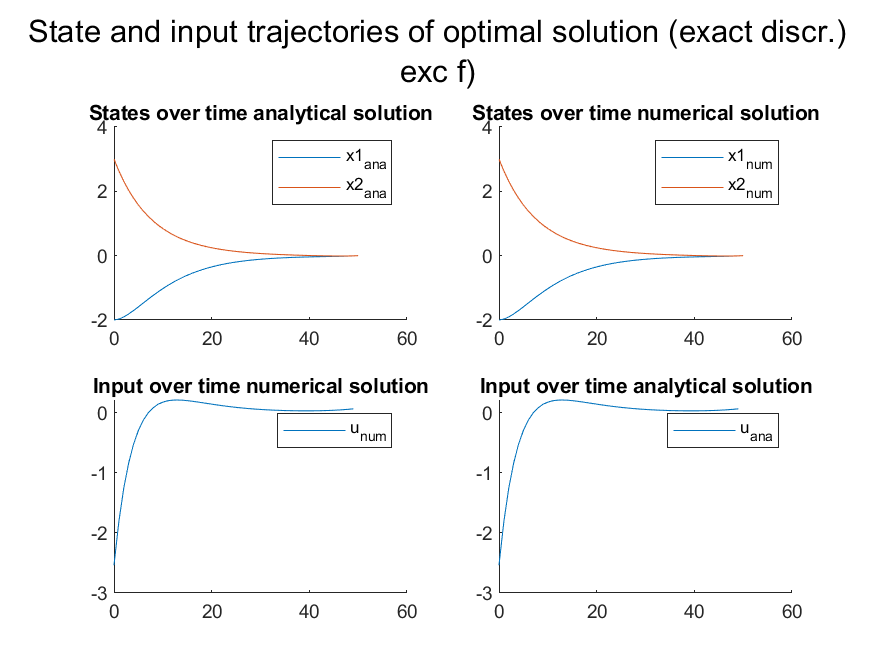
\includegraphics[width=0.95\linewidth]{plots/exc_f1.png}
	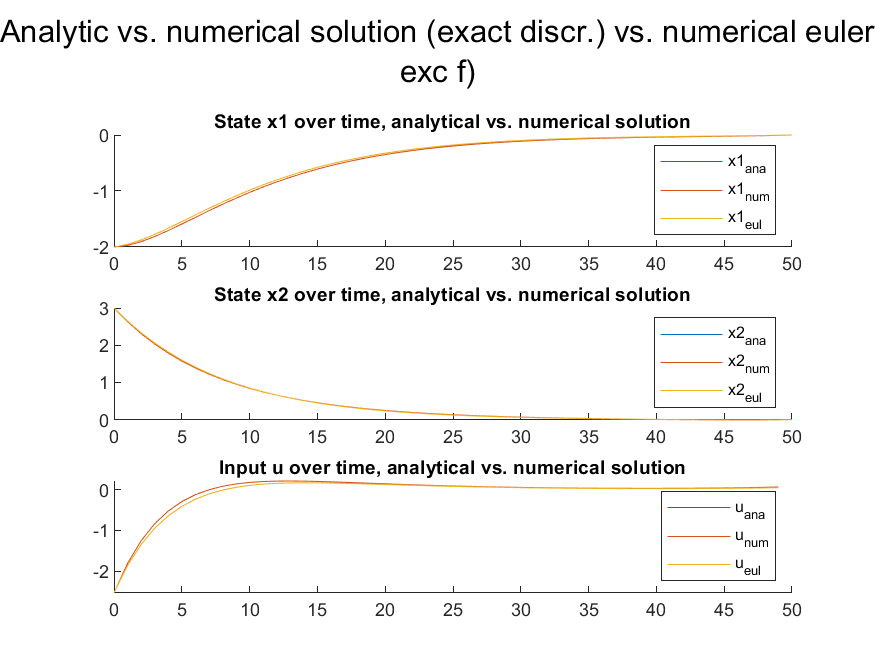
\includegraphics[width=0.95\linewidth]{plots/exc_f2.png}
	\caption{Plot for Exc f)}
	\label{fig:excf1}
\end{figure}
\begin{figure}[H]
	\centering
	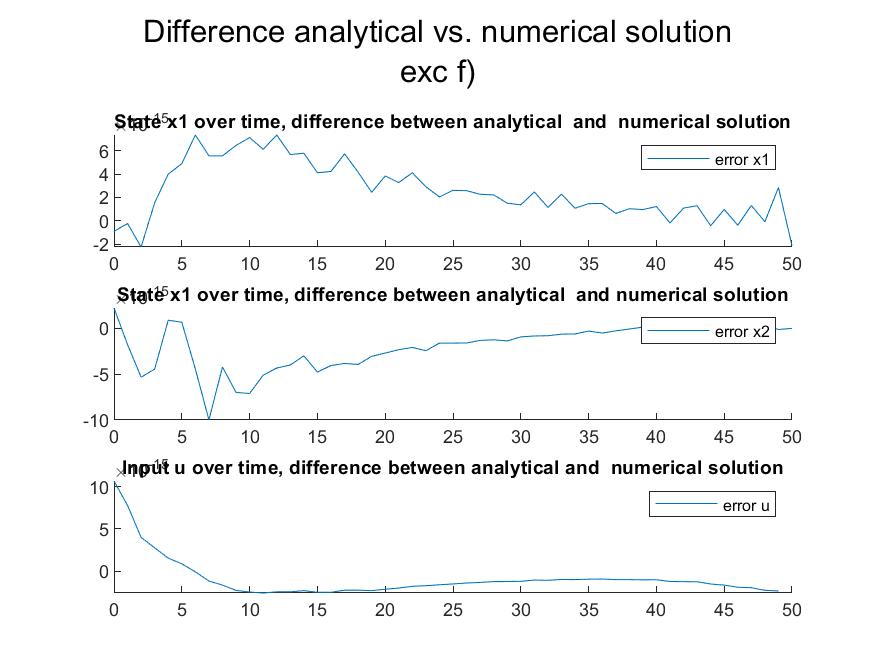
\includegraphics[width=0.95\linewidth]{plots/exc_f3.png}
	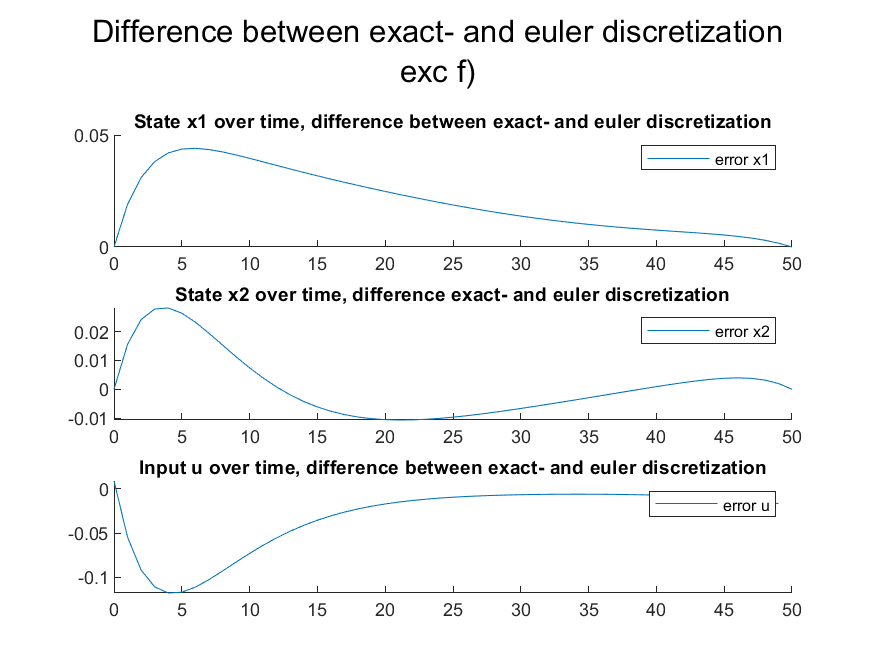
\includegraphics[width=0.95\linewidth]{plots/exc_f4.png}
	\caption{Plot for Exc f)}
	\label{fig:excf3}
\end{figure}

\subsection{Plots for g)}
\begin{figure}[H]
	\centering
	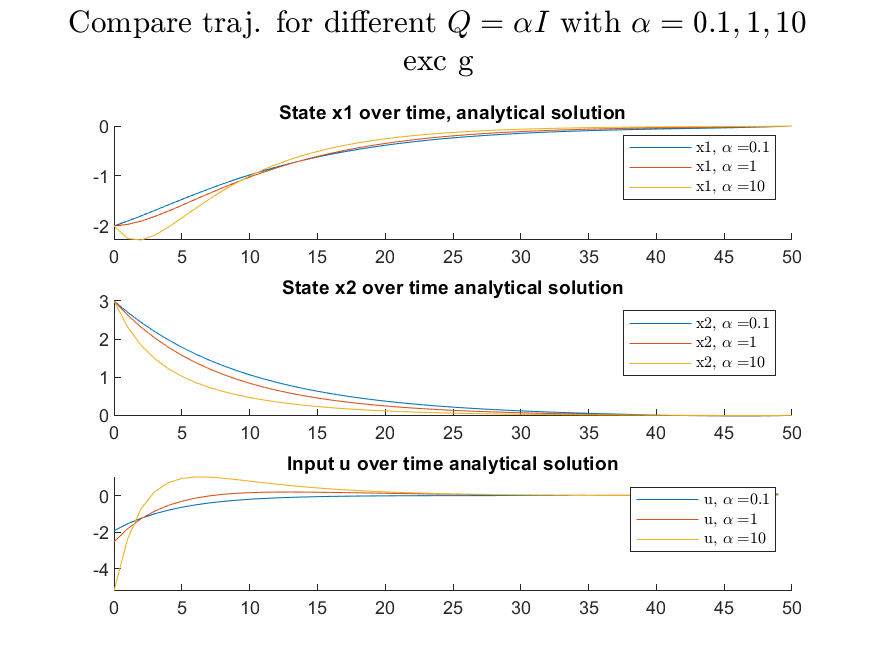
\includegraphics[width=0.95\linewidth]{plots/exc_g.png}
	\caption{Plot for Exc g)}
	\label{fig:excg}
\end{figure}

\subsection{Plots for h)}
\begin{figure}[H]
	\centering
	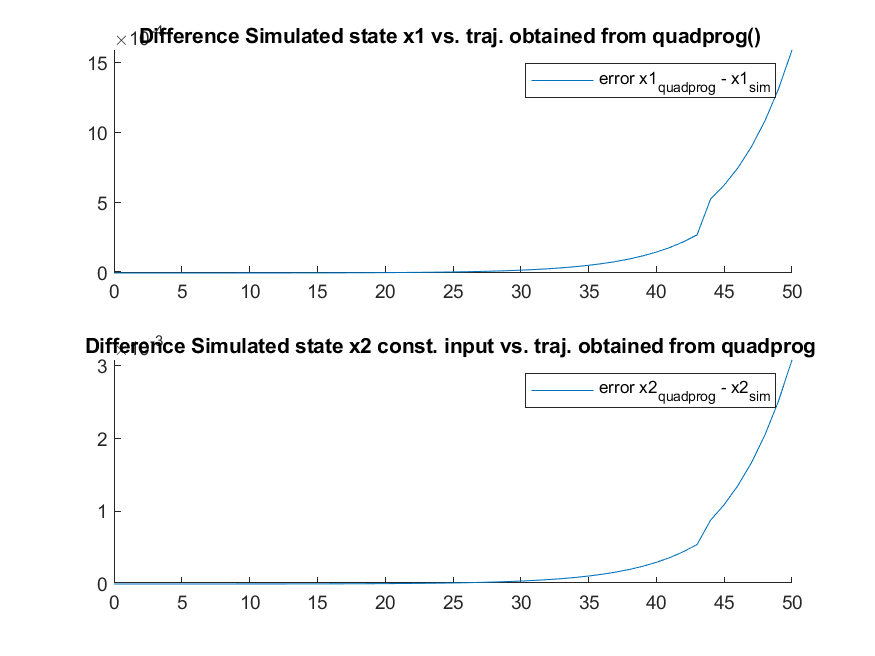
\includegraphics[width=0.95\linewidth]{plots/exc_h.png}
	\caption{Plot for Exc h)}
	\label{fig:exch}
\end{figure}




\end{document}
